\documentclass[10pt,a4paper,titlepage]{report}
\usepackage[latin1]{inputenc}
\usepackage{ucs}
\usepackage{amsmath}
\usepackage{amsfonts}
\usepackage{amssymb}
%\usepackage[dvips]{graphics}
\usepackage{graphics}
% Pour r�aliser un index
\usepackage{makeidx}
\makeindex
%%
\author{David Szerman}
\title{JDiveLog Manual}
\date{08th February 2006}
\begin{document}
\maketitle{}
\tableofcontents{}
\chapter{Licence informations}
JDiveLog is free software; you can redistribute it and/or modify it under the terms of the GNU General Public License as published by the Free Software Foundation; either version 2 of the License, or (at your option) any later version.

JDiveLog is distributed in the hope that it will be useful, but WITHOUT ANY WARRANTY; without even the implied warranty of MERCHANTABILITY or FITNESS FOR A PARTICULAR PURPOSE.  See the GNU General Public License for more details.

You should have received a copy of the GNU General Public License along with JDiveLog; if not, write to the Free Software Foundation, Inc., 59 Temple Place, Suite 330, Boston, MA  02111-1307  USA
\chapter{Introduction}
 JDiveLog is a logbook for scuba diving written in Java. It manages all important dive data, as well as the pictures taken during the dive. Features include import of UDCF data, data from Suunto/Uwatec computers, profile generation, web page generator.
You can also add pictures to your dives, see some statistics.
 
\chapter{Features}
JDiveLog software is made to store your dives and to replace your paper logbook.
You can
\begin{itemize}
\item edit dives, buddies, dive sites, activities and your equipment
\item export your book in order to include it on your website
\item import dives from your computer
\item import dives from different files
\item link pictures to your dives
\item see statistics about your dives
\item simulate your dives according to different decompression procedures (german, french,...)
\item use your software in different languages (french, english, german, finnish)
\end{itemize}
\chapter{General settings}
This is the first time you start our software ? Let's start with settings that can help you...

For this, go to the menu File > Settings > General.
From there, you can choose in which language you want to use the software (english, german, finnish or french), the units (metrics or imperial) and the date formats with and without time specification.
As it is said on the window : restart the software in order to apply the different new settings.\chapter{Edit the divelog  book}
From now, you can add some dives to your logbook... But first, you can add some dive places to the logbook. \section{Edit dive places}
You can edit the dive sites while you are editing a dive.

Go to the divesites tab and click on new site. A new window will open and you will be able to modify everything you want, such as the name, the country and other informations (ratings, comments). Once it is done, click on the close button.
If you want to delete a dive site, select the dive you want to erase and click on the Delete button.
\section{Edit buddies}
You can edit your buddies while you are editing a dive.

The same way, you can add buddies in order to be able to select them as often as you want.
Go to the menu Edit > Buddies list.
In order to insert a new buddy, insert his name and first name and click on New buddy.
In order to delete a buddyn the same way you deleted a dive place, you can select a buddy and click on the Delete button.

Once it is done, click on the close button.
\section {Add a dive}
Now, you are ready.

Go back to the main tab, called Logbook.

Click on the "Add a dive" button. A new window is now open with four tabs : Data, Equipment, Profile and Pictures.\subsection{Details}
This tab is the main tab with all dive informations. You can specify the date, time, max depth, min depth, average depth. In order to specify your buddies during this dive, you can specify them by writing their name manually. In this case, they will not be saved and you will not be able to see some statistics about them. 
The other way is to click on the "Add buddy" button and to insert a new buddy and/or select one buddy. If you want to select more than one, press the <CTRL> key while selecting the buddies.
You can act the same way to select the dive site.\subsection{Equipment}
\subsection{Profile}
This section is not manually editable ; the dive profile is created while importing the dives from files or directly from a dive computer.
\subsection{Pictures}
By clicking on the \textit{Add Pictures} button, a file browser will open.
You can select several pictures in the same directory by pressing the SHIFT or CTRL key.

Then you can modify the name of the picture, describe it, rate it  or rotate it. 
\chapter{Dive simulation}
\section{Warning}
This module is a simulation program which can not be used as dive planifier. \textbf{There is not any warranty for the calculation}. Use it as a demonstration, otherwise you will use it at your own risk.
\section{Simulation of a dive}
\subsection{Dive parameters}
First of all, you have to choose which decompression model you need to use.
You have choice between :
\begin{itemize}
\item Deco 2000 (german model) until 700 meters over the sea level
\item Deco 2000 (german model) from 700 to 1500 meters over the sea level
%\item MN90 (french model)
\end{itemize}
%\begin{figure}[htbp]
%	\centering
%		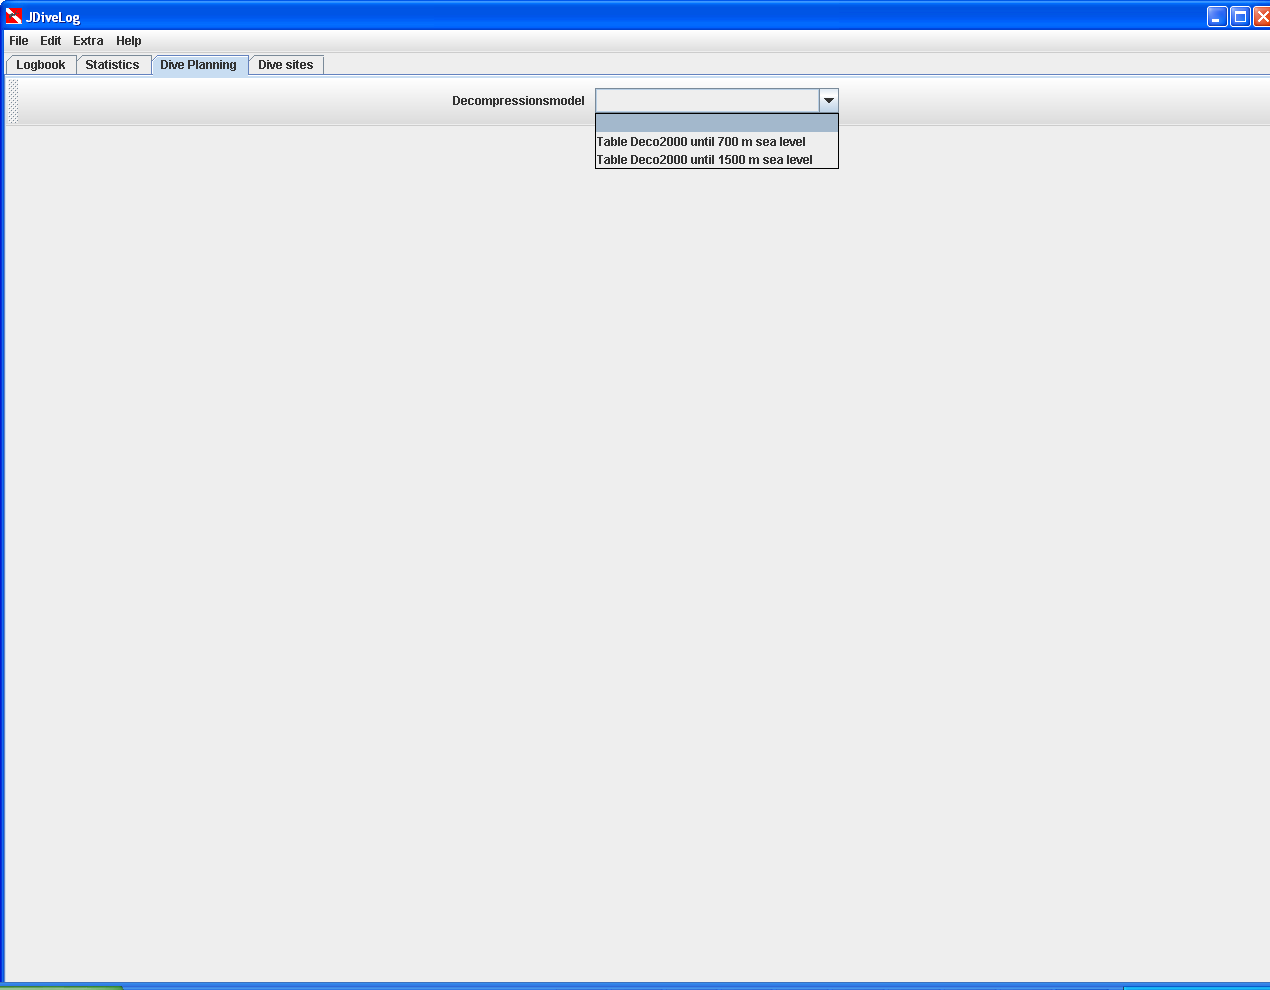
\includegraphics[width=0.80\textwidth]{./pictures/decoModelChoice.bb}
%	\caption{Choice of the decom\-pression model}
%	\label{fig:decoModelChoice}
%\end{figure}
Once you made your choice, you will arrive on the dive planifier with most of the fields empty.
%\begin{figure}
%	\centering
%		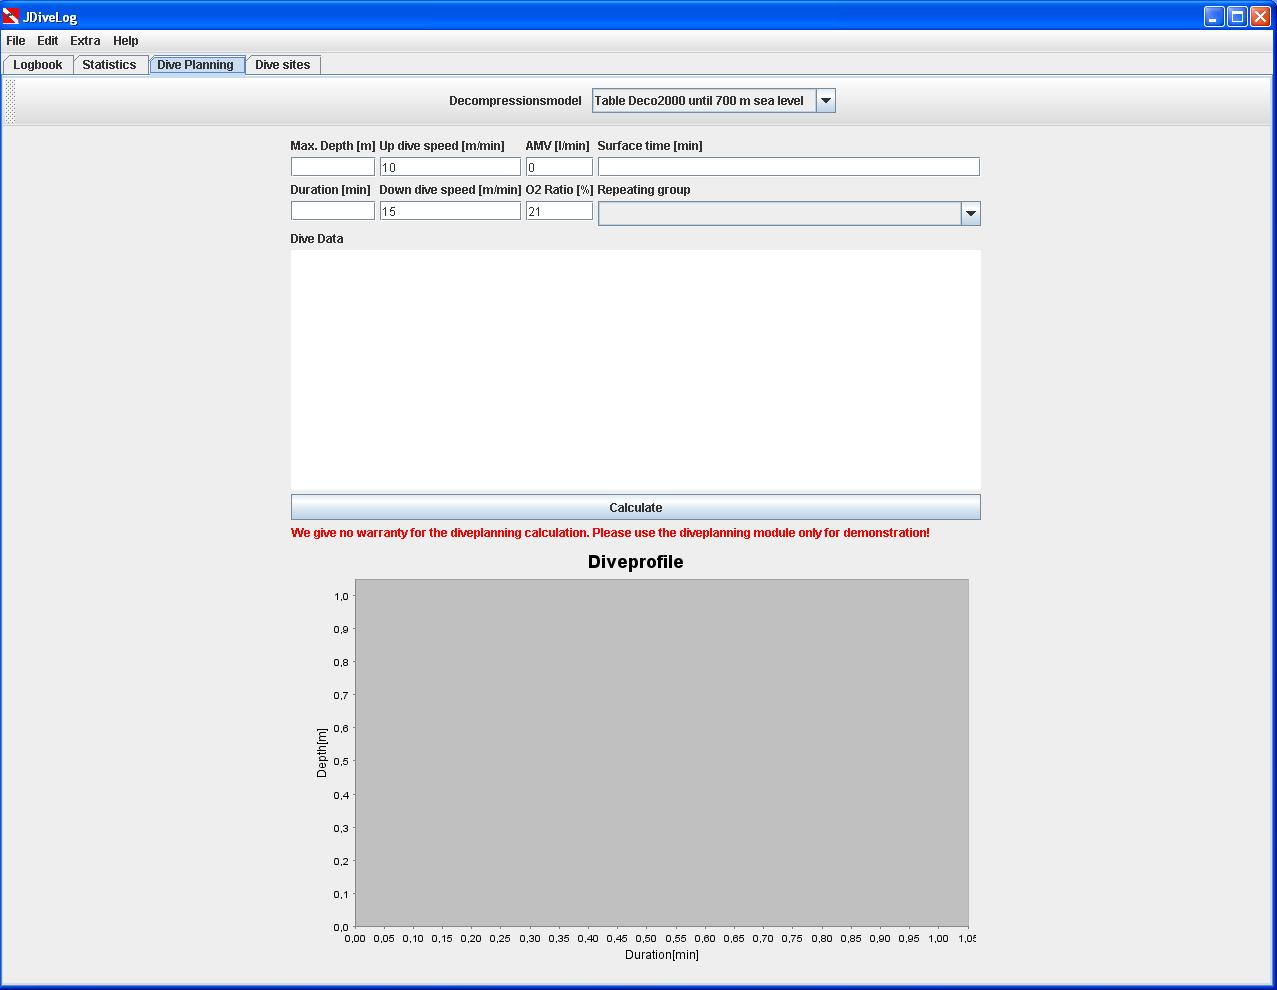
\includegraphics[width=0.95\textwidth]{./pictures/emptyDecoPlanifier.jpg}
%	\caption{Empty planifier}
%	\label{fig:emptyDecoPlanifier}
%\end{figure}

Let's fill them.

%\begin{figure}
%	\centering
%		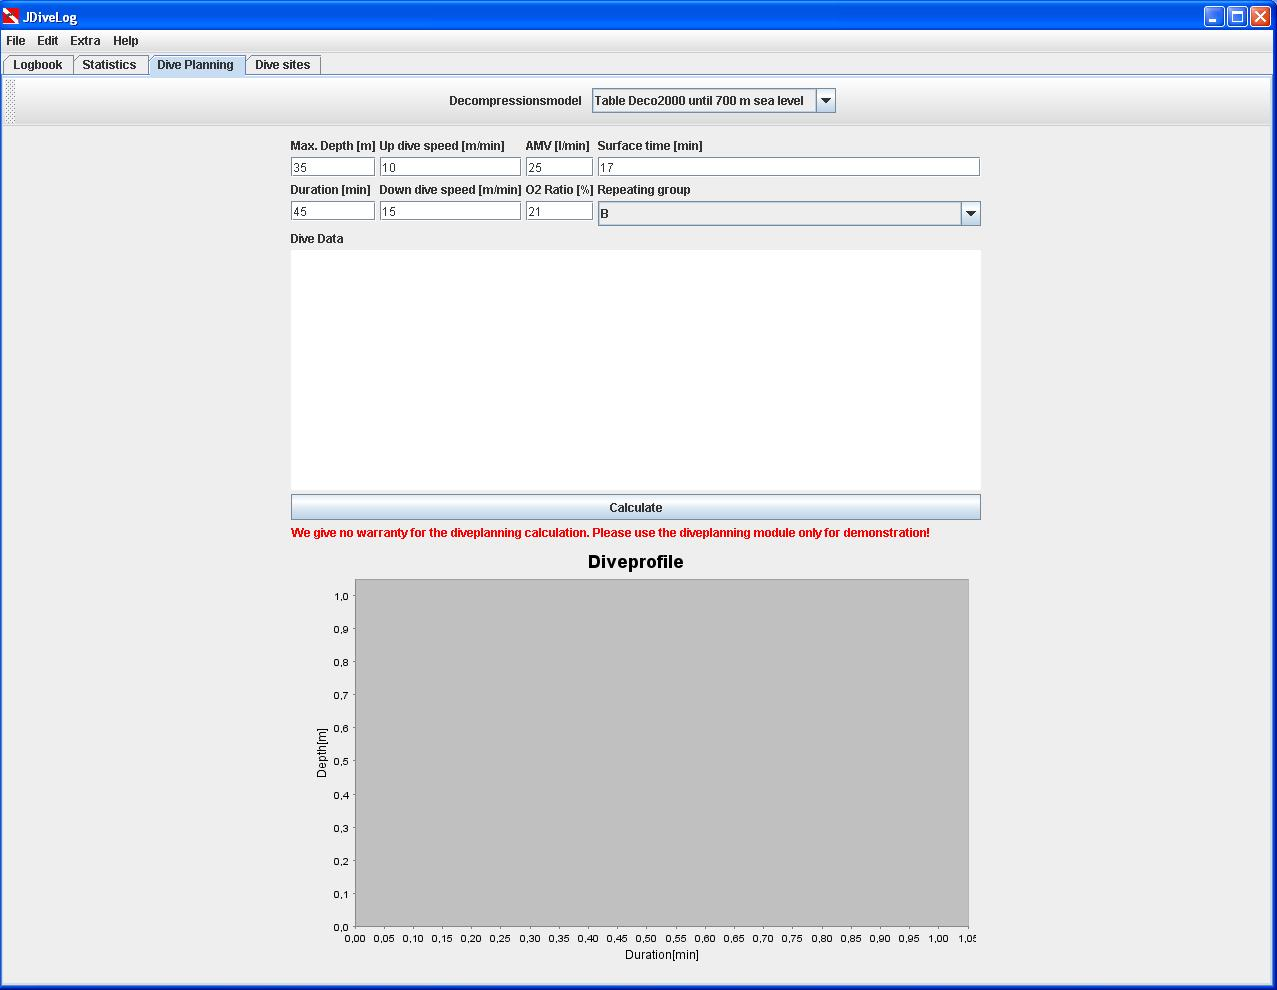
\includegraphics[width=0.95\textwidth]{./pictures/filledDecoPlanifier.jpg}
%	\caption{Empty planifier}
%	\label{fig:emptyDecoPlanifier}
%\end{figure}

Every data, \textbf{other than depth and duration}, which was not auto filled after you choosed the deco model is optionnal.
So you have to enter :
\begin{itemize}
	\item maximal depth
	\item bottom time
	\item up dive speed
	\item down dive speed
	\item $0_{2}$ percentage (for Nitrox mix).
\end{itemize}

If you made some dives before, you can specify :
\begin{itemize}
	\item the repeating group after the previous dive
	\item the surface time between the previous and the current dives.
\end{itemize}


Once it is done, click on \emph{Calculate}

\subsection{Results reading}

\chapter{Statistics}
\section{Settings}
\chapter{Import of the dives}
\section{Import from files}
You can import the dives and dive profiles from different kind of files.
\subsection{File formats supported}
\subsubsection{Suunto Dive Manager 2.x files}
From the Suunto Dive Manager software, choose to export in .SDE file type. For this, go to File > Export.
Once it is done, go to the JDiveLog's menu : File > Import SDM 2.x file 
Select the file you exported before and click on OK. Then select the dive(s) you want to insert.
Once it is done, you will see the dives in your logbook and will be able to edit them.
\subsubsection{Cressi PCLogBook exported files}
Importer is able to pull the data from Cressi Software CSV files including diving profile and basic dives information.
In main window of PCLogBook select the dives you want to export. You may select multiple items by holding "Ctrl" key and clicking them one by one. Then go to "File->Export" menu item. Ensure that "file csv(*.csv)" option is highlighted in "Save as type" section, enter the name of the file and save it.
After that click on "Import Cressi PC-Logbook file" under "File" menu in JDiveLog and select the CSV file.
You will be able to see the new data in your logbook.
\section{Import from dive computers}
\subsection{Computers supported}
\begin{itemize}
	\item Suunto VyTec
	\item Suunto VyTec DS
	\item Suunto Mosquito
	\item Suunto Stinger
	\item Suunto Cobra
	\item Suunto Vyper
	\item Suunto Gekko
	\item Uwatec Aladin Air Z/X
	\item Uwatec Aladin Air Z/X Nitrox
	\item Uwatec Aladin Air Z/X O2
	\item Uwatec Aladin Air
	\item Uwatec Aladin Sport
	\item Uwatec Aladin Pro
	\item Uwatec Aladin Pro Nitrox
	\item Spiro Monitor 2 Plus
	\item Spiro Monitor 3 Air
	\item Mares Genius
\end{itemize}
\subsection{Settings}
\subsection {Uwatec computers}
\subsection{Suunto computers}
To download profile data from your Suunto Computer make sure you have set the correct driver and settings in the Settings Menu
(choose Driver "Suunto VyTec, Vyper, Mosquito, Stinger", select the appropriate Com-Port / Device and choose the correct Model).
\begin{itemize}
	\item Open Settings from File-Menu
	\item Click on Divecomputer on the left side
	\item Choose Driver "Suunto VyTec, Vyper, Mosquito, Stinger"
	\item Select the appropriate Com-Port / Device
	\item Choose the correct Model (e.g. VyTec)
	\item Close the Settings window
	\item Start transfer on your Divecomputer (on the VyTec: Menu->Memory-TR-PC)
	\item Start Transfer in JDiveLog (press \textbf{F2} or the Button)
	\item Wait until all dives are transferred (Status is visible in the Statusbar on the bottom of JDiveLog
	\item When the Window with the profiles on your dive computer appears choose the dives you want to import (Note: the dives not yet in your logbook are marked as default)
	\item Press import and your dives will appear in your logbook
\end{itemize}
\chapter{Export of the log book}
\section{Settings}
\section{HTML files}

\chapter{Other Features}

\section{Search}
You can search for dives by pressing \textbf{ctrl-f}. The search syntax is very simple. You can specify one
or more search keywords to find all dives containing one of the specified words. For example searching for
'John Doe' would return dives with John Doe, John Smith and Peter Doe. If you want to search for dives with only John Doe
you would either prepend a '+' before each word such as '+John +Doe' or put John Doe in doublequotes like '"John Doe"'.
If you want to exclude a specific word from the list you could prepend a '-'.

\section{Slideshow}
To start a slideshow with your pictures of your logbook, you must select all dives containing the pictures you want to show
in your slideshow. You can select multiple dives by pressing \textbf{ctrl} while clicking on a dive. When you're finished selecting the
dives you can start the slideshow by pressing \textbf{F11}. While running the slideshow you can jump to the next picture by pressing \textbf{Page Dn}, \textbf{Space} or \textbf{enter}, to the previous picture by pressing \textbf{Page Up}. You can also rotate the image with the cursor-keys to left and right, edit the name (\textbf{F5}), the description (\textbf{F6}). To abort a running slideshow press \textbf{Esc}.
\chapter{Contributions}
Do you like JDiveLog? Do you want to request a feature? Translate the software or some parts of it? Develop some new features?
If you have any comments or suggestions, you can post a message in one of the forums \footnote{$http://sourceforge.net/forum/?group\_id=134952$}  or send an email to \textbf{pellmont@users.sourceforge.net}
\chapter{Conclusion}
\end{document}